\title{Mixture density networks}

\subsection{Mixture density networks}

We explore mixture density networks (MDN) \citep{bishop1994mixture}. We
demonstrate their implementation in Edward, leveraging Keras to
construct neural networks.

If you are not familiar with MDNs have a look at the
\href{http://cbonnett.github.io/MDN.html}{following blog post} or at
the original paper by \citet{bishop1994mixture}.
The script is available
\href{https://github.com/blei-lab/edward/blob/master/examples/tf_mixture_density_network_demo.py}
{here}.

\subsubsection{Data}

We use the same toy data from the
\href{http://blog.otoro.net/2015/11/24/mixture-density-networks-with-tensorflow/}{David
Ha's blog post}, where he explains MDNs. It is an inverse problem where
for every input $x_n$ there are multiple outputs $y_n$.

\begin{lstlisting}[language=Python]
def build_toy_dataset(N):
  y_data = np.random.uniform(-10.5, 10.5, (N, 1)).astype(np.float32)
  r_data = np.random.normal(size=(N, 1)).astype(np.float32)  # random noise
  x_data = np.sin(0.75 * y_data) * 7.0 + y_data * 0.5 + r_data * 1.0
  return train_test_split(x_data, y_data, random_state=42)

N = 40000  # number of data points
D = 1  # number of features

X_train, X_test, y_train, y_test = build_toy_dataset(N)
print("Size of features in training data: {:s}".format(X_train.shape))
print("Size of output in training data: {:s}".format(y_train.shape))
print("Size of features in test data: {:s}".format(X_test.shape))
print("Size of output in test data: {:s}".format(y_test.shape))

sns.regplot(X_train, y_train, fit_reg=False)
\end{lstlisting}

\begin{lstlisting}
## Size of features in training data: (4000, 1)
## Size of output in training data: (4000, 1)
## Size of features in test data: (36000, 1)
## Size of output in test data: (36000, 1)
\end{lstlisting}
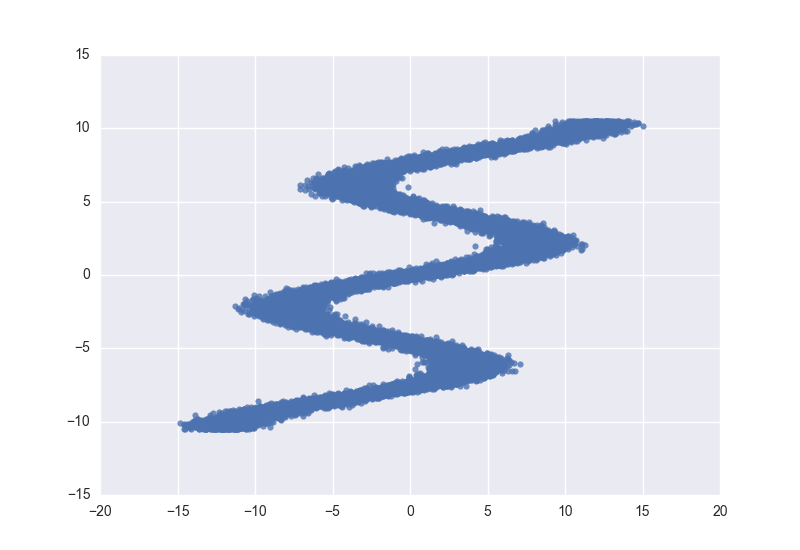
\includegraphics[width=700px]{/images/mdn-fig0.png}

We define TensorFlow placeholders will be used to manually feed batches of data during inference. This is \href{http://edwardlib.org/api/data}{one of many ways} to train models with data in Edward.

\begin{lstlisting}[language=Python]
X = tf.placeholder(tf.float32, [None, D])
y = tf.placeholder(tf.float32, [None, D])
data = {'X': X, 'y': y}
\end{lstlisting}


\subsubsection{Model}

\textbf{Note: Model wrappers are deprecated since Edward v1.1.5.
Reimplementing this under Edward's native language is currently in
progress.}

We define a class that can be used to construct MDNs. Here we use a
mixture of normal distributions parameterized by a feedforward
network. In other words, the membership probabilities and
per-component mean and standard deviation are given by the output of a
feedforward network.

\begin{lstlisting}[language=Python]
class MixtureDensityNetwork:
  """
  Mixture density network for outputs y on inputs x.

  p((x,y), (z,theta))
  = sum_{k=1}^K pi_k(x; theta) Normal(y; mu_k(x; theta), sigma_k(x; theta))

  where pi, mu, sigma are the output of a neural network taking x
  as input and with parameters theta. There are no latent variables
  z, which are hidden variables we aim to be Bayesian about.
  """
  def __init__(self, K):
    self.K = K

  def neural_network(self, X):
    """pi, mu, sigma = NN(x; theta)"""
    # fully-connected layer with 25 hidden units
    hidden1 = Dense(25, activation=K.relu)(X)
    hidden2 = Dense(25, activation=K.relu)(hidden1)
    self.mus = Dense(self.K)(hidden2)
    self.sigmas = Dense(self.K, activation=K.exp)(hidden2)
    self.pi = Dense(self.K, activation=K.softmax)(hidden2)

  def log_prob(self, xs, zs):
    """Return scalar, the log joint density log p(xs, zs)."""
    # Note there are no parameters we're being Bayesian about. The
    # parameters are baked into how we specify the neural networks.
    X, y = xs['X'], xs['y']
    self.neural_network(X)
    result = self.pi * norm.prob(y, self.mus, self.sigmas)
    result = tf.log(tf.reduce_sum(result, 1))
    return tf.reduce_sum(result)
\end{lstlisting}

We instantiate the mixture density network with 20 mixtures.

\begin{lstlisting}[language=Python]
model = MixtureDensityNetwork(20)
\end{lstlisting}

\subsubsection{Inference}

We use MAP estimation, passing
in the model and data set.
See this extended tutorial about
\href{/tutorials/map}{MAP estimation in Edward}.

\begin{lstlisting}[language=Python]
inference = ed.MAP([], data, model)
\end{lstlisting}

Here, we will manually control the inference and how data is passed
into it at each step. First, start a TensorFlow session and pass it
into Keras so that it shares the same TensorFlow session as Edward.
Then initialize the algorithm and the TensorFlow variables.

\begin{lstlisting}[language=Python]
sess = ed.get_session()
K.set_session(sess)
inference.initialize()

init = tf.global_variables_initializer()
init.run()
\end{lstlisting}

Now we train the MDN by calling \texttt{inference.update()}, passing
in the data. The quantity \texttt{inference.loss} is the
loss function (negative log-likelihood) at that step of inference. We
also report the loss function on test data by calling
\texttt{inference.loss} and where we feed test data to the TensorFlow
placeholders instead of training data.
We keep track of the losses under \texttt{train\_loss} and \texttt{test\_loss}.

\begin{lstlisting}[language=Python]
n_epoch = 1000
train_loss = np.zeros(n_epoch)
test_loss = np.zeros(n_epoch)
for i in range(n_epoch):
    info_dict = inference.update(feed_dict={X: X_train, y: y_train})
    train_loss[i] = info_dict['loss']
    test_loss[i] = sess.run(inference.loss, feed_dict={X: X_test, y: y_test})
\end{lstlisting}

After training for a number of iterations,
we can get out the predictions we are interested in from
the model. In this case, it is

\begin{itemize}
\item
\texttt{model.pi}, the mixture components;
\item
\texttt{model.mus}, the means;
\item
\texttt{model.sigmas}, the standard deviations.
\end{itemize}

To do this, we call
\begin{lstlisting}[language=Python]
pred_weights, pred_means, pred_std = \
    sess.run([model.pi, model.mus, model.sigmas], feed_dict={X: X_test})
\end{lstlisting}

Let's plot the log-likelihood of the training and test data as
functions of the training epoch. The quantity \texttt{inference.loss}
is the total log-likelihood, not the loss per data point.  In the
plotting routine we get the latter by dividing by the size of the
train and test data respectively.

\begin{lstlisting}[language=Python]
fig, axes = plt.subplots(nrows=1, ncols=1, figsize=(16, 3.5))
plt.plot(np.arange(n_epoch), -test_loss / len(X_test), label='Test')
plt.plot(np.arange(n_epoch), -train_loss / len(X_train), label='Train')
plt.legend(fontsize=20)
plt.xlabel('Epoch', fontsize=15)
plt.ylabel('Log-likelihood', fontsize=15)
\end{lstlisting}

\includegraphics[width=700px]{/images/mdn-fig1.png}

We see that it converges after 400 iterations.

\subsubsection{Criticism}

Let's look at how a few individual examples perform. Note that as this
is an inverse problem we can't get the answer correct, but we can hope
that the truth lies in area where the model has high probability. This code relies on helper functions
available in the full script above.

In this plot the truth is the vertical grey line while the blue line is the prediction of the mixture density network. As you can see, we didn't do too bad.

\begin{lstlisting}[language=Python]
obj = [0, 4, 6]
fig, axes = plt.subplots(nrows=3, ncols=1, figsize=(16, 6))

plot_normal_mix(pred_weights[obj][0], pred_means[obj][0], pred_std[obj][0], axes[0], comp=False)
axes[0].axvline(x=y_test[obj][0], color='black', alpha=0.5)

plot_normal_mix(pred_weights[obj][2], pred_means[obj][2], pred_std[obj][2], axes[1], comp=False)
axes[1].axvline(x=y_test[obj][2], color='black', alpha=0.5)

plot_normal_mix(pred_weights[obj][1], pred_means[obj][1], pred_std[obj][1], axes[2], comp=False)
axes[2].axvline(x=y_test[obj][1], color='black', alpha=0.5)
\end{lstlisting}

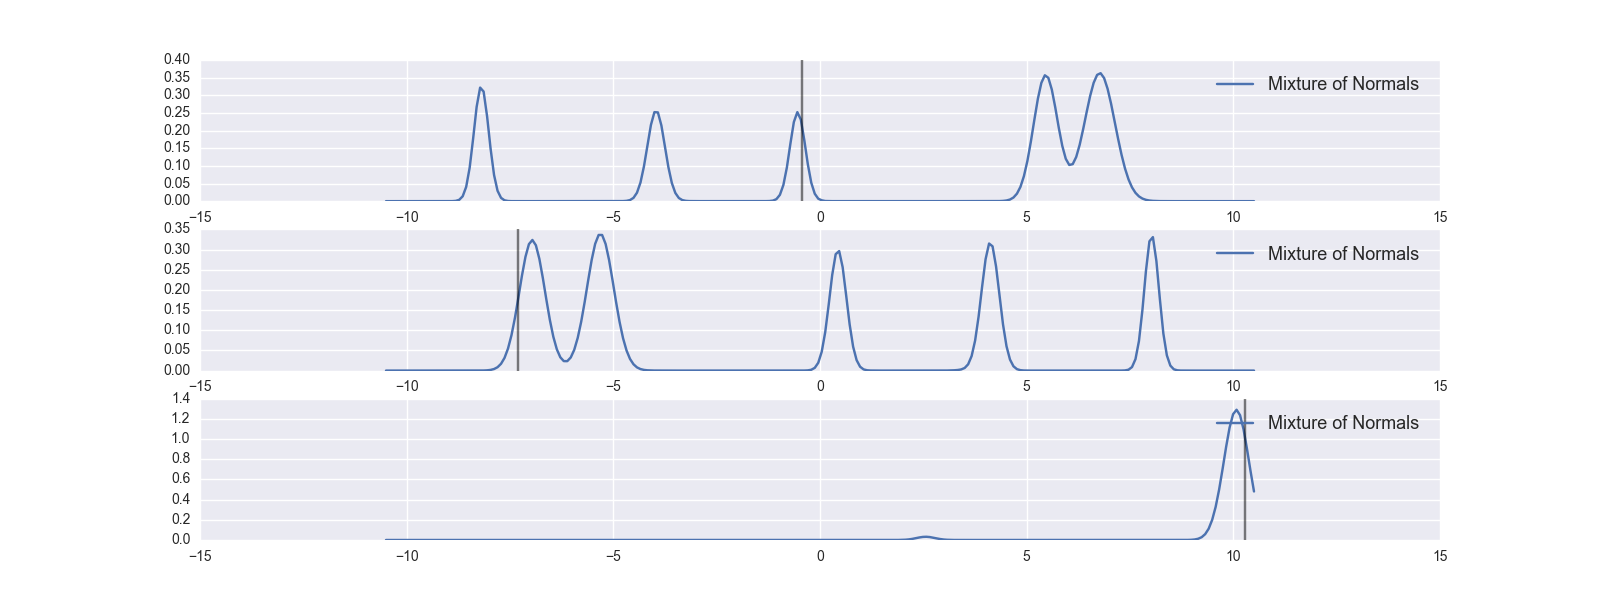
\includegraphics[width=700px]{/images/mdn-fig2.png}

We can check the ensemble by drawing samples of the prediction and
plotting the density of those. The MDN has learned what we'd like it
to learn.

\begin{lstlisting}[language=Python]
a = sample_from_mixture(X_test, pred_weights, pred_means, pred_std, amount=len(X_test))
sns.jointplot(a[:,0], a[:,1], kind="hex", color="#4CB391", ylim=(-10,10), xlim=(-14,14))
\end{lstlisting}

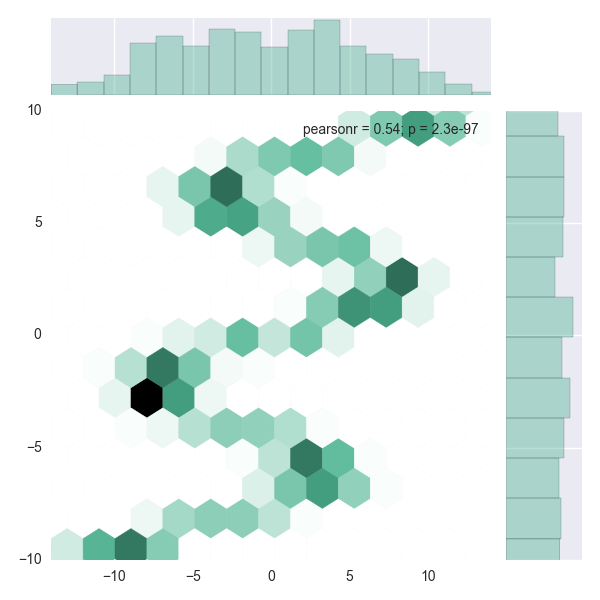
\includegraphics[width=700px]{/images/mdn-fig3.png}

\subsubsection{Acknowledgments}

We are grateful to Christopher Bonnett for writing this tutorial, and
more generally for pushing forward momentum to have Edward tutorials
be accessible and easy-to-learn.

\subsubsection{References}\label{references}
